% !TEX program = xelatex
\documentclass[11pt]{article}
\usepackage{graphicx,fontspec,geometry,hyperref,float}
\usepackage[bottom]{footmisc}
\geometry{
	a4paper,
	top=2.5cm,
	bottom=2cm,
	left=2cm,
	right=2cm
}
% Justify Paragrapher
\newcommand{\justified}
{
	\tolerance=1
	\emergencystretch=\maxdimen
	\hyphenpenalty=10000
	\hbadness=10000
}


\graphicspath{ {./images/} }
\setmainfont{Times New Roman}
%%%%%%%%%%%%%%%%%%%%%%%%%%%%%%%%%%%%%%%%%%%%%%%%%%%%%%%%

\title{
	\vspace{-2cm}
	\textbf{Artificial Neural Network and Deep Learning}\\
	\large Homework 2
}
\date{}

\author{Angelo Capponcelli \and Pasquale Castiglione \and Mehdi Samimi}

\begin{document}
\maketitle
\justified

\section*{Dataset}
\subsection*{Data Exploration}
Not having enough information about the dataset, we performed data exploration. In particular, after printing the summary statistics, we plotted the distribution of the classes and some random samples in order to extract something valuable.
\subsection*{Class Imbalance}
From the histogram of the of the classes, a problem of class imbalance was spotted. We tried to overcome this problem using different techniques. Firstly we tried to set the \emph{class\_weight} parameter in the \emph{Model.fit()} function, then we tried to random \emph{oversample} the smaller classes adding noise to the new samples and finally we tried \emph{data augmentation} using the library \emph{tsaug\footnote{\url{https://tsaug.readthedocs.io/en/stable/}}}.\\
Unfortunately none of the approaches listed above gave us the desired results, so we stayed with the original dataset.

\subsection*{Preprocessing}
The dataset was firstly shuffled and then split into training set and validation set. During development a ratio of 75/25 turned out to be the best choice. In the data exploration phase we observed that values were widely scattered from $-10000$ to $+50000$ so we decided to standardize\footnote{$X_{new} = \frac{X - \mu}{\sigma} $} them in order to shift and scale the input into a distribution having mean 0 with standard deviation 1. We performed the standardization directly inside the model adding a \emph{keras.layers.Normalization} layer after the input layer. For this computation we used the mean and the variance of the training dataset.

\begin{figure}[H]
\center
	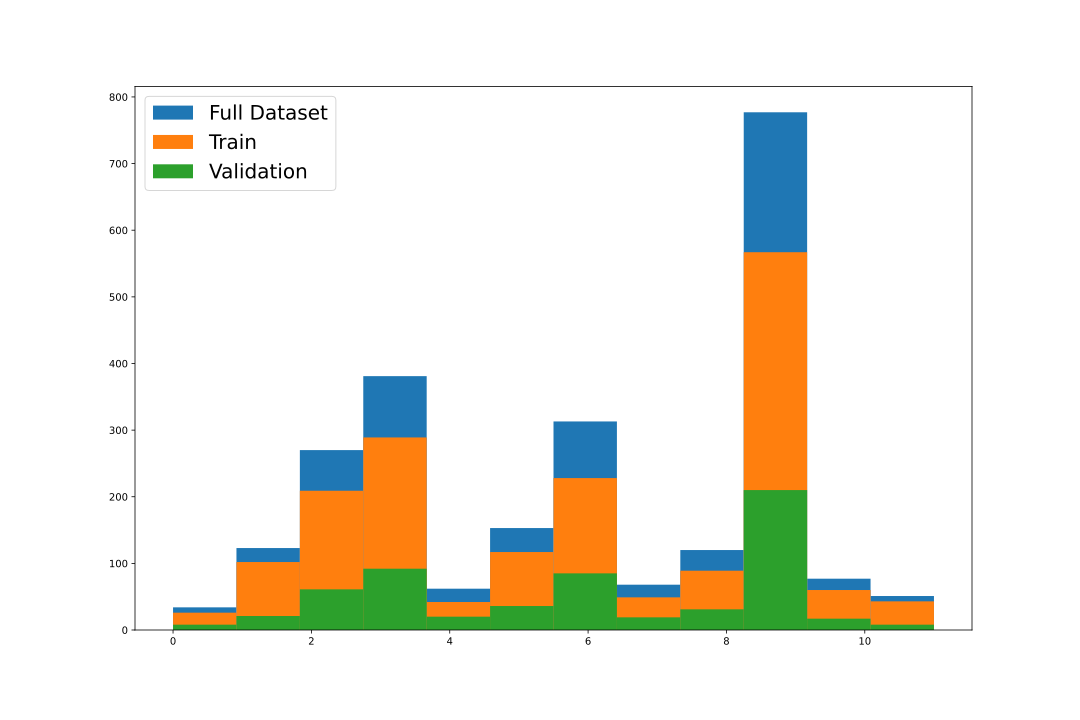
\includegraphics[scale=0.4]{class_histogram.png}
	\caption{Histogram of the classes}
\end{figure}


\section*{Model Development}
\subsection*{First Models}
We started with a simple model composed of a stack of three blocks each one containing a \emph{Conv1D} layers with 128 filters of 3x3 each, followed by a \emph{MaxPooling1D} layer. The last block was directly connected to the output layer. This first model led us to an accuracy of $\approx 0.65$.\\
Willing to improve the accuracy score we made the model more complex by adding two \emph{Bidirectional LSTM} with 128 units each just before the output layer. This latter approach led us to an accuracy score of $\approx0.69$. 
\subsection*{Overfitting}
As the accuracy score went up, the model started to suffer overfitting so, in order to overcome this, we implemented some expedients.\\
Firstly we added a \emph{Dropout} layer with a rate of 0.5 just before the output layer, then we reduced the units of the LSTM layers from 128 to 100, then we added a \emph{Dropout} layer with a rate of 0.3 after each convolutional block and finally we set the \emph{recurrent\_regularizer} parameter in the LSTMs to \emph{keras.regularizers.L1L2(1e-2, 1e-2)}. After some trials, keeping only one \emph{Bidirectional LSTM} showed better result so we decided to remove the second one. After using all of these, we were able to reduce the overfitting but also to increase the accuracy.


\subsection*{Final Model}
Therefore the final model was composed of a feature extraction part, a recurrent part and the output layer:
\begin{itemize}
	\item\textbf{Feature Extraction Part:} Composed of a stack of three blocks, each one composed of a \emph{Conv1D}, a \emph{MaxPooling1D} and a \emph{Dropout}.
	\item\textbf{Recurrent Part:} Consisted of a \emph{Bidirectional LSTM} layer with 100 units by a \emph{Dropout} layer.
	\item\textbf{Output:} A single dense layer with 12 units and a softmax activation function.
\end{itemize}


\begin{figure}[H]
\center
	\includegraphics[scale=0.35]{model_summary.png}
	\caption{Summary of the Final Model}
\end{figure}

\section*{Training}
For the training, after some experiments, a \emph{batch\_size} of 64 resulted to be the right trade off between overfitting and accuracy. The training lasted 100 epochs and we made use of two callbacks: \emph{early stopping} with a patience of 10 in order to avoid overfitting and to reduce waste of time and \emph{ReduceLROnPlateau} with a patience of 5 and a minimum learning rate of 1e-6 to improve the learning.
With all these tweaks, we were able to reach an accuracy score of $\approx0.72$  on the training dataset and an accuracy score of $\approx0.73$ on the test set in Codalab.

\begin{figure}[H]
\center
	\includegraphics[width=\textwidth]{accuracy.png}
	\caption{Accuracy}
\end{figure}

\subsection*{Conclusion}
The model turned out to be pretty much robust, showing the same behavior with both the training set and test set. Furthermore it was also a relatively simple model that allowed to have little training times.

\end{document}
